% Options for packages loaded elsewhere
\PassOptionsToPackage{unicode}{hyperref}
\PassOptionsToPackage{hyphens}{url}
\PassOptionsToPackage{dvipsnames,svgnames,x11names}{xcolor}
%
\documentclass[
  letterpaper,
  DIV=11,
  numbers=noendperiod]{scrartcl}

\usepackage{amsmath,amssymb}
\usepackage{iftex}
\ifPDFTeX
  \usepackage[T1]{fontenc}
  \usepackage[utf8]{inputenc}
  \usepackage{textcomp} % provide euro and other symbols
\else % if luatex or xetex
  \usepackage{unicode-math}
  \defaultfontfeatures{Scale=MatchLowercase}
  \defaultfontfeatures[\rmfamily]{Ligatures=TeX,Scale=1}
\fi
\usepackage{lmodern}
\ifPDFTeX\else  
    % xetex/luatex font selection
\fi
% Use upquote if available, for straight quotes in verbatim environments
\IfFileExists{upquote.sty}{\usepackage{upquote}}{}
\IfFileExists{microtype.sty}{% use microtype if available
  \usepackage[]{microtype}
  \UseMicrotypeSet[protrusion]{basicmath} % disable protrusion for tt fonts
}{}
\makeatletter
\@ifundefined{KOMAClassName}{% if non-KOMA class
  \IfFileExists{parskip.sty}{%
    \usepackage{parskip}
  }{% else
    \setlength{\parindent}{0pt}
    \setlength{\parskip}{6pt plus 2pt minus 1pt}}
}{% if KOMA class
  \KOMAoptions{parskip=half}}
\makeatother
\usepackage{xcolor}
\setlength{\emergencystretch}{3em} % prevent overfull lines
\setcounter{secnumdepth}{-\maxdimen} % remove section numbering
% Make \paragraph and \subparagraph free-standing
\makeatletter
\ifx\paragraph\undefined\else
  \let\oldparagraph\paragraph
  \renewcommand{\paragraph}{
    \@ifstar
      \xxxParagraphStar
      \xxxParagraphNoStar
  }
  \newcommand{\xxxParagraphStar}[1]{\oldparagraph*{#1}\mbox{}}
  \newcommand{\xxxParagraphNoStar}[1]{\oldparagraph{#1}\mbox{}}
\fi
\ifx\subparagraph\undefined\else
  \let\oldsubparagraph\subparagraph
  \renewcommand{\subparagraph}{
    \@ifstar
      \xxxSubParagraphStar
      \xxxSubParagraphNoStar
  }
  \newcommand{\xxxSubParagraphStar}[1]{\oldsubparagraph*{#1}\mbox{}}
  \newcommand{\xxxSubParagraphNoStar}[1]{\oldsubparagraph{#1}\mbox{}}
\fi
\makeatother


\providecommand{\tightlist}{%
  \setlength{\itemsep}{0pt}\setlength{\parskip}{0pt}}\usepackage{longtable,booktabs,array}
\usepackage{calc} % for calculating minipage widths
% Correct order of tables after \paragraph or \subparagraph
\usepackage{etoolbox}
\makeatletter
\patchcmd\longtable{\par}{\if@noskipsec\mbox{}\fi\par}{}{}
\makeatother
% Allow footnotes in longtable head/foot
\IfFileExists{footnotehyper.sty}{\usepackage{footnotehyper}}{\usepackage{footnote}}
\makesavenoteenv{longtable}
\usepackage{graphicx}
\makeatletter
\def\maxwidth{\ifdim\Gin@nat@width>\linewidth\linewidth\else\Gin@nat@width\fi}
\def\maxheight{\ifdim\Gin@nat@height>\textheight\textheight\else\Gin@nat@height\fi}
\makeatother
% Scale images if necessary, so that they will not overflow the page
% margins by default, and it is still possible to overwrite the defaults
% using explicit options in \includegraphics[width, height, ...]{}
\setkeys{Gin}{width=\maxwidth,height=\maxheight,keepaspectratio}
% Set default figure placement to htbp
\makeatletter
\def\fps@figure{htbp}
\makeatother

\KOMAoption{captions}{tableheading}
\makeatletter
\@ifpackageloaded{caption}{}{\usepackage{caption}}
\AtBeginDocument{%
\ifdefined\contentsname
  \renewcommand*\contentsname{Tabla de contenidos}
\else
  \newcommand\contentsname{Tabla de contenidos}
\fi
\ifdefined\listfigurename
  \renewcommand*\listfigurename{Listado de Figuras}
\else
  \newcommand\listfigurename{Listado de Figuras}
\fi
\ifdefined\listtablename
  \renewcommand*\listtablename{Listado de Tablas}
\else
  \newcommand\listtablename{Listado de Tablas}
\fi
\ifdefined\figurename
  \renewcommand*\figurename{Figura}
\else
  \newcommand\figurename{Figura}
\fi
\ifdefined\tablename
  \renewcommand*\tablename{Tabla}
\else
  \newcommand\tablename{Tabla}
\fi
}
\@ifpackageloaded{float}{}{\usepackage{float}}
\floatstyle{ruled}
\@ifundefined{c@chapter}{\newfloat{codelisting}{h}{lop}}{\newfloat{codelisting}{h}{lop}[chapter]}
\floatname{codelisting}{Listado}
\newcommand*\listoflistings{\listof{codelisting}{Listado de Listados}}
\makeatother
\makeatletter
\makeatother
\makeatletter
\@ifpackageloaded{caption}{}{\usepackage{caption}}
\@ifpackageloaded{subcaption}{}{\usepackage{subcaption}}
\makeatother

\ifLuaTeX
\usepackage[bidi=basic]{babel}
\else
\usepackage[bidi=default]{babel}
\fi
\babelprovide[main,import]{spanish}
% get rid of language-specific shorthands (see #6817):
\let\LanguageShortHands\languageshorthands
\def\languageshorthands#1{}
\ifLuaTeX
  \usepackage{selnolig}  % disable illegal ligatures
\fi
\usepackage{bookmark}

\IfFileExists{xurl.sty}{\usepackage{xurl}}{} % add URL line breaks if available
\urlstyle{same} % disable monospaced font for URLs
\hypersetup{
  pdftitle={U6. Impuestos a los consumos},
  pdfauthor={Sebastian Freille},
  pdflang={es},
  colorlinks=true,
  linkcolor={blue},
  filecolor={Maroon},
  citecolor={Blue},
  urlcolor={Blue},
  pdfcreator={LaTeX via pandoc}}


\title{U6. Impuestos a los consumos}
\usepackage{etoolbox}
\makeatletter
\providecommand{\subtitle}[1]{% add subtitle to \maketitle
  \apptocmd{\@title}{\par {\large #1 \par}}{}{}
}
\makeatother
\subtitle{Finanzas Públicas}
\author{Sebastian Freille}
\date{}

\begin{document}
\maketitle


\section{\texorpdfstring{\textbf{Bibliografia}}{Bibliografia}}\label{bibliografia}

\begin{itemize}
\tightlist
\item
  Albi, E., González-Páramo, J. M., \& Zubiri, I. (2009). Economía
  Pública II (3ra. edición). Barcelona: Ariel. Capítulos 7. Solicitar
  por: T 336 A 53015 T.2
\item
  Rosen, H. S. (2008). Hacienda Pública (7ma. edición). Madrid:
  McGraw-Hill/Interamericana. Capítulo 19, págs 475 a 493.
\end{itemize}

\subsection{Programa Analítico}\label{programa-analuxedtico}

\begin{enumerate}
\def\labelenumi{\arabic{enumi}.}
\item
  Unidad 1.La economía del sector público: Introducción, conceptos y
  alcance
\item
  Unidad 2. Las decisiones colectivas: Agregación de preferencias y
  decisiones sociales
\item
  Unidad 3. El gasto público. El presupuesto público.
\item
  Unidad 4. Los recursos del sector público.
\item
  Unidad 5. Impuestos a los ingresos
\item
  \textbf{Unidad 6. Impuestos a los consumos}
\item
  Unidad 7. Impuestos a la riqueza y otros impuestos.
\item
  Unidad 8. Sostenibilidad fiscal: déficit público, endeudamiento y
  emisión monetaria.
\item
  Unidad 9. Federalismo fiscal y relaciones financieras
  inter-gubernamentales
\item
  Unidad 10. Temas especiales: Tributación y gasto internacional,
  sistemas de pensiones y programas de redistribución
\end{enumerate}

\section{\texorpdfstring{\textbf{Unidad 6. Impuestos a los
consumos}}{Unidad 6. Impuestos a los consumos}}\label{unidad-6.-impuestos-a-los-consumos}

\section{\texorpdfstring{\textbf{Introducción: aspectos
generales}}{Introducción: aspectos generales}}\label{introducciuxf3n-aspectos-generales}

\subsection{Preguntas}\label{preguntas}

\begin{itemize}
\item
  ¿Gravar a la renta o a los consumos no es lo mismo?
\item
  ¿La imposición al consumo distorsiona la decisión consumo-ahorro?
\item
  ¿Qué tipos de impuestos al consumo existen?
\item
  ¿Son eficientes y equitativos los impuestos al consumo?
\item
  ¿Por qué son atractivos los impuestos al consumo
\end{itemize}

\section{\texorpdfstring{\textbf{Ingreso versus
consumo}}{Ingreso versus consumo}}\label{ingreso-versus-consumo}

\begin{itemize}
\tightlist
\item
  El consumo es otra manifestación de capacidad contributiva, tal como
  lo es el ingreso o el patrimonio.
\item
  Podría ser instrumentado entonces un principio de equidad donde los
  que más consuman más paguen -- progresividad. Para ello se requeriría
  gravar en forma directa el consumo --impuesto al gasto total de las
  personas en bienes de consumo.
\item
  En términos de eficiencia, la diferencia fundamental entre un impuesto
  a la renta y un impuesto al consumo es que el segundo no distorsiona
  la decisión consumo/ahorro.
\item
  En otras palabras, esta forma de imposición consiste en gravar el
  \textbf{consumo real} en lugar del \textbf{consumo potencial}
  --recuerde que \(Y=C+S\)
\end{itemize}

\begin{center}\rule{0.5\linewidth}{0.5pt}\end{center}

\begin{itemize}
\tightlist
\item
  Sabemos que: \[\begin{aligned}
          C+S=Y \\
          C=Y-S
        \end{aligned}\]
\item
  ¿Qué pasa con la renta que se ahorra? Dos personas pueden ganar lo
  mismo pero consumir una mas que la otra. Con un impuesto a la Y
  pagarían lo mismo, con un impuesto al C pagarian diferente.
\item
  En otras palabras, ¿debemos eximir al ahorro del pago de impuestos?
  \(\longrightarrow\) equivale a preguntar si debe eximirse los ingresos
  generados por el ahorro (intereses, dividendos, ganancias de capital)
\end{itemize}

\section{\texorpdfstring{\textbf{Tipos de imposición al
consumo}}{Tipos de imposición al consumo}}\label{tipos-de-imposiciuxf3n-al-consumo}

Los impuestos al consumo pueden ser:

\begin{itemize}
\tightlist
\item
  De carácter personal

  \begin{itemize}
  \tightlist
  \item
    Impuesto al gasto
  \end{itemize}
\item
  De carácter no personal

  \begin{itemize}
  \tightlist
  \item
    Determinados bienes

    \begin{itemize}
    \tightlist
    \item
      Impuestos específicos
    \end{itemize}
  \item
    Consumo en general

    \begin{itemize}
    \tightlist
    \item
      Impuesto generales sobre las ventas
    \end{itemize}
  \end{itemize}
\end{itemize}

\begin{center}\rule{0.5\linewidth}{0.5pt}\end{center}

\begin{figure}[H]

{\centering 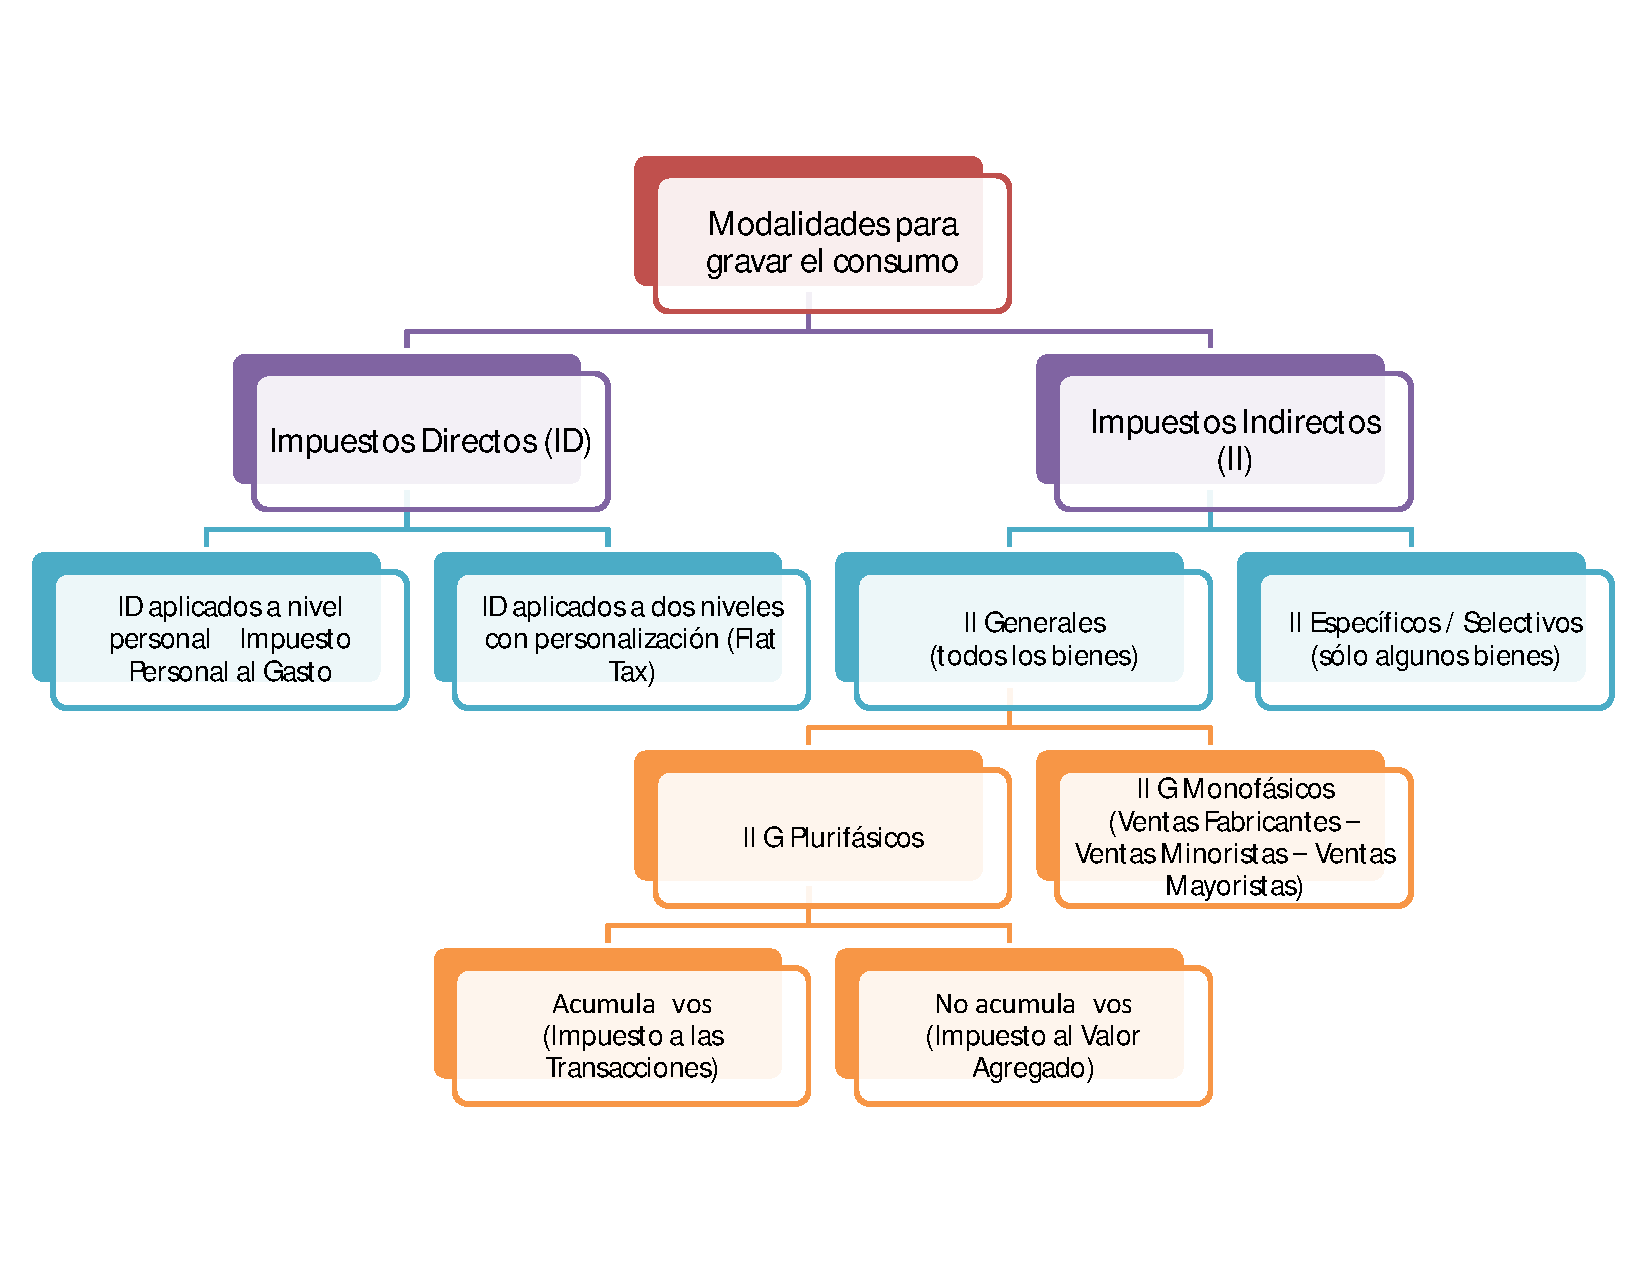
\includegraphics{../_shared/images/fpub/uni6_tiposconsumo.pdf}

}

\caption{Modalidades de imposición al consumo}

\end{figure}%

\section{\texorpdfstring{\textbf{Enfoques para gravar el
consumo}}{Enfoques para gravar el consumo}}\label{enfoques-para-gravar-el-consumo}

\begin{itemize}
\tightlist
\item
  Imposición directa sobre el gasto personal \(\longrightarrow\) se
  aplica un impuesto sobre los gastos que realizan las familias en
  bienes de consumo --no alcanza el ahorro, salvo cuando éste es
  consumido
\item
  Imposición proporcional sobre la renta con exención del rendimiento
  normal del ahorro \(\longrightarrow\) se aplica un impuesto sobre la
  renta que exime expresamente el rendimiento normal del ahorro.
\item
  Imposición proporcional sobre la renta con desgravación de la
  inversión de capital \(\longrightarrow\) Se aplica un impuesto sobre
  la renta que permite deducir el 100\% de las inversiones realizadas,
  en el mismo momento en que éstas se realizan. Luego, cuando la
  inversión se realiza se grava por el total de la misma. Este impuesto
  generaría los mismos efectos que un impuesto al consumo
\item
  Imposición indirecta sobre el consumo (mercado de bienes)
\end{itemize}

\section{\texorpdfstring{\textbf{Ingreso versus consumo: Efectos sobre
ahorro}}{Ingreso versus consumo: Efectos sobre ahorro}}\label{ingreso-versus-consumo-efectos-sobre-ahorro}

\begin{quote}
Dos gemelos idénticos Modesto y Presunto, ambos ganan lo mismo a lo
largo de la vida. Sin embargo, Modesto ahorra el 20\% de sus ingresos
durante su vida y logra acumular un ahorro importante para su
jubilación. Presunto gasta todo su ingreso y cuando se jubila debe
acudir al Estado. Si hay un impuesto a la renta, Modesto pagará mucho
más impuesto que Presunto --debe pagar impuestos sobre los intereses que
generan sus ahorros) y recibe mucho menos prestaciones. Obviamente,
Modesto no esetará muy contento con esta situación ya que percibe que se
penaliza el ahorro (ingreso futuro).
\end{quote}

\section{\texorpdfstring{\textbf{Equivalencia de
impuestos}}{Equivalencia de impuestos}}\label{equivalencia-de-impuestos}

\begin{itemize}
\tightlist
\item
  Se dice que dos impuestos son equivalentes si su incidencia es
  exactamente la misma --impuesto sobre el consumo e impuesto sobre el
  salario equivalentes
\item
  Que dos impuestos sean equivalentes no implica que no haya efectos
  cuando se sustituye uno por otro --equivalencia en este sentido
  implica \textbf{mismos efectos a largo plazo}
\item
  Ejemplo \(\longrightarrow\) si se sustituye un impuesto sobre el \(Y\)
  a lo largo de toda la vida por un impuesto sobre el \(C\) a lo largo
  de toda la vida, los ancianos deberán pagar impuestos dos veces!
\end{itemize}

\begin{center}\rule{0.5\linewidth}{0.5pt}\end{center}

\begin{itemize}
\tightlist
\item
  Ejemplos de impuestos equivalentes

  \begin{itemize}
  \tightlist
  \item
    Impuestos sobre la renta e impuestos sobre el valor agregado (sin
    excención de inversión)
  \item
    Impuestos sobre el consumo e impuestos sobre el valor agregado (con
    excención de inversión)
  \item
    Impuestos sobre el consumo e impuestos sobre los salarios
  \item
    Impuestos sobre la renta y el consumo de toda la vida (sin
    donaciones ni herencias)
  \end{itemize}
\end{itemize}

\section{\texorpdfstring{\textbf{Ingreso durante toda la
vida}}{Ingreso durante toda la vida}}\label{ingreso-durante-toda-la-vida}

\begin{itemize}
\tightlist
\item
  ¿Qué pasaria si en vez de pagar impuesto a la renta anual lo pagaramos
  por todo el período de ingresos de la vida? \(\longrightarrow\) el Y
  obtenido a lo largo de la vida es el \emph{valor actual descontado} de
  los ingresos salariales del individuo
\item
  Si una persona vive durante dos períodos y recibe un salario \(w_0\)
  en el primero y \(w_1\) en el segundo, el valor actual descontado
  sera: \[y*=w_0+\frac{w_1}{1+r}\]
\item
  Y notese que el valor descontado del consumo de esa persona a lo largo
  de su vida debe ser igual al valor descontado del ingreso (si no hay
  herencias, donaciones.
\end{itemize}

\begin{center}\rule{0.5\linewidth}{0.5pt}\end{center}

\begin{itemize}
\tightlist
\item
  En otras palabras, si \(c_0\) es el consumo en el primer período y
  \(c_1\) el consumo en en l segundo período, entonces:
  \[y*=c_0+\frac{c_1}{1+r}\]
\item
  Puede comprobarse que si la base tributaria es el ingreso a lo largo
  de su vida entonces es lo mismo que hacer que la base tributaria sea
  el consumo a lo largo de toda su vida.
\item
  Independientemente de cómo se reparta la renta o el consumo, pagarían
  lo mismo si se cumpliera lo anterior \(\longrightarrow\) no afecta
  decisión consumo ahorro.
\item
  Implicancia \(\longrightarrow\) la renta procedente de intereses debe
  estar exenta!
\end{itemize}

\subsection{Incentivos: Decisión
consumo-ahorro}\label{incentivos-decisiuxf3n-consumo-ahorro}

\begin{itemize}
\tightlist
\item
  Dos períodos --1 y 2- y dos casos --A y B. La alícuota es igual a
  \(t=10\%\).
\item
  Sean \(Y_1=100\), \(Y_2=0\) y la tasa de interés, \(i=10\%\).
  SUPUESTO: No hay ahorro al final de la vida.
\item
  Casos alternativos de uso del ingreso:

  \begin{itemize}
  \tightlist
  \item
    Caso A (gastador miope) \(\longrightarrow\) \(Y_1=C_1=100\) e
    \(Y_2=C_2=0\)
  \item
    Caso B (ahorrador ascético) \(\longrightarrow\) \(Y_1=100\),
    \(C_1=0\) e \(Y_2=10\), \(C_2=110\)
  \end{itemize}
\item
  Veamos que pasa con los impuestos al consumo e impuesto al ingreso en
  ambos casos.
\end{itemize}

\begin{center}\rule{0.5\linewidth}{0.5pt}\end{center}

\begin{itemize}
\tightlist
\item
  \textbf{Impuesto al consumo}

  \begin{itemize}
  \tightlist
  \item
    Caso A \(\longrightarrow\) impuesto en período 1, \(T_1=C_1*t\) es
    decir \(T_1=100*0.1=10\); impuesto en período 2, \(T_2=C_2*t\) es
    decir \(T_2=0*0.1=0\). \(T_1\) llevado al período 2 con interés es
    igual a \(11\). Impuesto total: \(T_1+T_2=11\)
  \item
    Caso B \(\longrightarrow\) impuesto en período 1, \(T_1=C_1*t\) es
    decir \(T_1=0*0.1=0\); impuesto en período 2, \(T_2=C_2*t\) es decir
    \(T_2=110*0.1=11\). Impuesto total: \(T_1+T_2=11\)
  \end{itemize}
\end{itemize}

\begin{center}\rule{0.5\linewidth}{0.5pt}\end{center}

\begin{itemize}
\tightlist
\item
  \textbf{Impuesto al ingreso}

  \begin{itemize}
  \tightlist
  \item
    Caso A \(\longrightarrow\) impuesto en período 1, \(T_1=Y_1*t\) es
    decir \(T_1=100*0.1=10\); impuesto en período 2, \(T_2=Y_2*t\) es
    decir \(T_2=0*0.1=0\). \(T_1\) llevado al período 2 con interés es
    igual a \(11\). Impuesto total: \(T_1+T_2=11\)
  \item
    Caso B \(\longrightarrow\) impuesto en período 1, \(T_1=Y_1*t\) es
    decir \(T_1=100*0.1=10\); impuesto en período 2, \(T_2=Y_2*t\) es
    decir \(T_2=10*0.1=1\). \(T_1\) llevado al periodo 2 con interes es
    igual a \(11\). Impuesto total: \(T_1+T_2=11+1=12\)
  \end{itemize}
\item
  Puede observarse como el impuesto al consumo no distorsiona la
  decisión consumo-ahorro mientras que el impuesto a la renta si lo hace
  --i.e.~conviene consumir todo antes y no ahorrar nada.
\end{itemize}

\section{\texorpdfstring{\textbf{Impuesto personal al
gasto}}{Impuesto personal al gasto}}\label{impuesto-personal-al-gasto}

\begin{itemize}
\tightlist
\item
  Permite gravar una manifestación de capacidad contributiva aplicando
  progresividad. Posibilidad de deducciones y aspectos específicos de
  las familias. Puede definirse un criterio ``amplio'' o ``estrecho'' de
  consumo --el último incluiría donaciones y herencias dadas.
\item
  Sujeción espacial \(\longrightarrow\) para garantizar equidad entre
  contribuyentes la potestad tributaria debería recaer en el país donde
  reside la persona y gravarse los consumos hechos en el país y fuera
  del país.
\item
  Delimitación temporal \(\longrightarrow\) Por ser variable flujo, debe
  definirse el período sobre el que se van a acumular los gastos para
  determinar la base del impuesto.
\item
  Unidad contribuyente \(\longrightarrow\) Enfoque individual vs
  familiar. Mismos problemas de incentivos que en impuesto a la renta.
\item
  Su gran problema es la complejidad administrativa.
\end{itemize}

\section{\texorpdfstring{\textbf{Impuesto plano: Flat
Tax}}{Impuesto plano: Flat Tax}}\label{impuesto-plano-flat-tax}

Combina dos impuestos: - Un impuesto sobre las empresas
\(\longrightarrow\) base consiste en las ventas netas de materias
primas, materiales, insumos, inversiones, sueldos y jornales. Como se
permite restar las inversiones en el momento en que se realizan, el
impuesto se asemeja en sus efectos a un impuesto que grava el consumo
(se desgrava el rendimiento normal de las inversiones). - Un impuesto
sobre las personas \(\longrightarrow\) base son los
sueldos/salarios/jubilaciones, incluyendo una deducción personal. - Se
aplica con alícuota plana sobre ambos niveles, aunque también podrían
aplicarse alícuotas progresivas. - Ventajas \(\longrightarrow\) grava
una sola vez los distintos tipos de rentas; simplicidad administrativa;
capacidad recaudadora.

\section{\texorpdfstring{\textbf{Impuestos indirectos: Impuesto a las
transacciones}}{Impuestos indirectos: Impuesto a las transacciones}}\label{impuestos-indirectos-impuesto-a-las-transacciones}

\begin{itemize}
\tightlist
\item
  Gravan el consumo en forma indirecta. Poco usado en el mundo excepto
  en...Argentina! \(\longrightarrow\) impuesto a los ingresos brutos.
\item
  Grava las \textbf{ventas} de todos los productos y en todas las fases
  de la producción y comercialización \(\longrightarrow\) es por ello
  que es de carácter general y plurifásico.
\item
  Genera el famoso \textbf{efecto cascada} (o efecto acumulación)
  \(\longrightarrow\) grava ventas brutas de distintas etapas.
\item
  La BI se conforma de las ventas del contribuyente acumuladas durante
  un período de tiempo determinado; puede aplicarse con alícuota única
  (la misma alícuota para todas las etapas) o con alícuotas
  diferenciales (usualmente crecientes hacia el consumo final)
\end{itemize}

\section{\texorpdfstring{\textbf{Impuestos indirectos: Efecto
acumulación
(``cascada'')}}{Impuestos indirectos: Efecto acumulación (``cascada'')}}\label{impuestos-indirectos-efecto-acumulaciuxf3n-cascada}

\begin{figure}[H]

{\centering \includegraphics{../_shared/images/fpub/uni6_cascada.pdf}

}

\caption{Valor agregado y efecto cascada}

\end{figure}%

\subsection{Impuesto a las transacciones:
Eficiencia}\label{impuesto-a-las-transacciones-eficiencia}

\begin{itemize}
\tightlist
\item
  Presenta muchas deficiencias desde el punto de vista de la eficiencia.
  Entre sus desventajas estan:

  \begin{itemize}
  \tightlist
  \item
    Genera cambios en precios relativos \(\longrightarrow\) bienes mas
    gravados aquellos de mas etapas
  \item
    Lesiona la competitividad externa de bienes de exportación
  \item
    Penaliza a los bienes de producción nacional que compiten con
    importaciones
  \item
    Grava doblemente a los bienes de K --cuando se venden y cuando se
    incorporan como insumos al proceso productivo.
  \item
    Incentiva integracion vertical de las empresas
  \end{itemize}
\item
  Tampoco es un buen impuesto desde el punto de vista de la equidad
  \(\longrightarrow\) incide más fuerte sobre aquellos que más consumen
\item
  ¿Por qué se usa entonces? Amplísima base imponible permite alícuotas
  bajas; baja visibilidad ante votantes/consumidores; facil de recaudar.
\end{itemize}

\subsection{Impuestos indirectos
monofásicos}\label{impuestos-indirectos-monofuxe1sicos}

\begin{itemize}
\tightlist
\item
  Existen impuestos indirectos de tipo \textbf{monofásicos}
  \(\longrightarrow\) gravan sólo una etapa del proceso de producción.
  Algunos ejemplos son el Impuesto a las Ventas Mayoristas o Impuesto a
  las Ventas Minoristas (IVM).
\item
  La BI va creciendo a medida que se llega a las etapas finales por lo
  que permite usar alicuotas bajas para obtener mayor recaudación (o
  misma recaudación con menor alícuota)
\item
  Desde la eficiencia \(\longrightarrow\) el ``mejor'' sería un Impuesto
  a las Ventas Finales (IVF) {[}¿Por qué?{]}
\item
  El IVF grava solo ventas para consumo final; a diferencia del IVM que
  podría gravar bienes no destinados a consumo final.
\item
  Desventaja del IVF \(\longrightarrow\) dificil control, fiscalización
  y ``ocultamiento'' de ventas finales
\end{itemize}

\section{\texorpdfstring{\textbf{Impuestos monofásicos:
Ejemplos}}{Impuestos monofásicos: Ejemplos}}\label{impuestos-monofuxe1sicos-ejemplos}

\begin{figure}[H]

{\centering \includegraphics{../_shared/images/fpub/uni6_monofasicos.pdf}

}

\caption{Comparación de impuestos monofásicos}

\end{figure}%

\section{\texorpdfstring{\textbf{Impuestos indirectos monofásicos:
resumen}}{Impuestos indirectos monofásicos: resumen}}\label{impuestos-indirectos-monofuxe1sicos-resumen}

\begin{itemize}
\tightlist
\item
  Para un mismo tipo impositivo, el efecto es mayor sobre el precio
  cuanto más nos acercamos a la fase minorista, pero la recaudación
  también es mayor.
\item
  Los monofásicos minoristas son más neutrales. El impacto en el precio
  no depende del número de fases de producción y distribución.
\item
  Los monofásicos no permiten una ajuste en frontera adecuado (salvo el
  minorista)
\item
  En los monofásicos es difícil delimitar quienes son fabricante,
  mayorista o minorista. Ademas, el control cruzado no es posible.
\end{itemize}

\section{\texorpdfstring{\textbf{Impuesto al valor
agregado}}{Impuesto al valor agregado}}\label{impuesto-al-valor-agregado}

\begin{figure}[H]

{\centering \includegraphics{../_shared/images/fpub/uni6_valoragregado.pdf}

}

\caption{La cadena de valor agregado}

\end{figure}%

\begin{center}\rule{0.5\linewidth}{0.5pt}\end{center}

\begin{itemize}
\tightlist
\item
  En un proceso productivo se obtiene un producto \(Y\) con una
  tecnología \(F\) a partir de insumos \(x_i\) usando trabajo \(L\) y
  capital \(K\). El \textbf{valor agregado (VA)} es lo que se añade a
  los insumos en el proceso y que se incorpora al producto
\item
  Con las ventas del producto \(Y\) se logran recursos para pagar: 1) el
  gasto en insumos; 2) el VA --este último corresponde a salarios
  pagados, a la retribución al \(K\) y a los beneficios
  empresariales/profesionales
\item
  El valor agregado bruto (VAB) es pues: \begin{align}
  VAB=B+wL+(\rho+\delta)K=pY-\sum_{i=1}^{n}q_{i}x_{i}
  \end{align}
\end{itemize}

\begin{center}\rule{0.5\linewidth}{0.5pt}\end{center}

\begin{itemize}
\item
  Es un impuesto indirecto sobre el consumo que grava las ventas de
  bienes en general, en todas sus etapas, pero que es no acumulativo
  \(\longrightarrow\) la BI es el valor agregado en cada etapa. El VA en
  toda etapa puede determinarse a partir de dos métodos:

  \begin{itemize}
  \item
    por adición --suma de pagos a los factores
  \item
    por sustracción --diferencia entre valor de venta del bien en etapa
    ``i'' y el valor de insumos adquiridos en etapa ``i'. En este
    método, hay dos variantes: a) sustracción real --diferencia valor
    producido menos insumos usados (requiere valuar inventarios); b)
    sustracción financiera --valor de ventas menos valor de compra de
    insumos.
  \end{itemize}
\item
  El problema de las diferencias entre estos tres metodos se dan a corto
  plazo y generalmente por la variación de existencias (acumulación de
  stocks insumos/productos)
\end{itemize}

\subsection{El impuesto al valor agregado
(cont.)}\label{el-impuesto-al-valor-agregado-cont.}

\begin{itemize}
\item
  En la práctica hay dos métodos de cálculo operativo frecuentemente
  usados.

  \begin{itemize}
  \item
    IVA metodo valor añadido bruto \(\longrightarrow\) valor agregado
    como diferencia entre valor de ventas y valor de compras de insumos
    y bienes de K: \(VA_i=Vtas_{i}-Cpras_{i}\)
  \item
    IVA método credito en el impuesto \(\longrightarrow\) el IVA a
    ingresar por una empresa es igual al IVA facturado en sus ventas
    menos el IVA soportado en sus compras: \(VA_i=IVA_i^V-IVA_i^C\)
  \end{itemize}
\end{itemize}

\subsection{IVA en relación a otros impuestos
indirectos}\label{iva-en-relaciuxf3n-a-otros-impuestos-indirectos}

\begin{itemize}
\item
  Ventajas respecto a otros multifasicos

  \begin{itemize}
  \item
    reparte su carga con uniformidad con independencia del numero de
    fases
  \item
    no crea ``rentas fiscales''
  \end{itemize}
\item
  Ventajas respecto a monofasico sobre minoristas

  \begin{itemize}
  \item
    No es preciso definir que se entiende por minorista
  \item
    Facilita mas informacion a la administracion tributaria
  \end{itemize}
\end{itemize}




\end{document}
